%%%%%%%%%%%%%%%%%%%%%%%%%%%%%%%%%%%%%%%%%%%%%%%%%%%%%%%%
%                IAML 2020 Assignment 2                %
%                                                      %
%                                                      %
% Authors: Hiroshi Shimodaira and JinHong Lu           %
% Based on: Assignment 1 by Oisin Mac Aodha, and       %
%          Octave Mariotti                             %
% Using template from: Michael P. J. Camilleri and     %
% Traiko Dinev.                                        %
%                                                      %
% Based on the Cleese Assignment Template for Students %
% from http://www.LaTeXTemplates.com.                  %
%                                                      %
% Original Author: Vel (vel@LaTeXTemplates.com)        %
%                                                      %
% License:                                             %
% CC BY-NC-SA 3.0                                      %
% (http://creativecommons.org/licenses/by-nc-sa/3.0/)  %
%                                                      %
%%%%%%%%%%%%%%%%%%%%%%%%%%%%%%%%%%%%%%%%%%%%%%%%%%%%%%%%

%--------------------------------------------------------
%   IMPORTANT: Do not touch anything in this part
\documentclass[12pt]{article}
%%%%%%%%%%%%%%%%%%%%%%%%%%%%%%%%%%%%%%%%%
% Cleese Assignment
% Structure Specification File
% Version 1.0 (27/5/2018)
%
% This template originates from:
% http://www.LaTeXTemplates.com
%
% Author:
% Vel (vel@LaTeXTemplates.com)
%
% License:
% CC BY-NC-SA 3.0 (http://creativecommons.org/licenses/by-nc-sa/3.0/)
% 
%%%%%%%%%%%%%%%%%%%%%%%%%%%%%%%%%%%%%%%%%

%----------------------------------------------------------------------------------------
%	PACKAGES AND OTHER DOCUMENT CONFIGURATIONS
%----------------------------------------------------------------------------------------

\usepackage{lastpage} % Required to determine the last page number for the footer
\usepackage{graphicx} % Required to insert images
\setlength\parindent{0pt} % Removes all indentation from paragraphs
\usepackage[most]{tcolorbox} % Required for boxes that split across pages
\usepackage{booktabs} % Required for better horizontal rules in tables
\usepackage{listings} % Required for insertion of code
\usepackage{etoolbox} % Required for if statements
\usepackage{geometry} % Required for adjusting page dimensions and margins
\usepackage[utf8]{inputenc} % Required for inputting international characters
\usepackage[T1]{fontenc} % Output font encoding for international characters
\usepackage{fancyhdr} % Required for customising headers and footers
\usepackage{xspace}
\usepackage{booktabs}
\usepackage[colorlinks]{hyperref}
\usepackage{etoolbox}

\newcommand{\ie}{i.e.\@\xspace}
\newcommand{\eg}{e.g.\@\xspace}
\newcommand{\notemark}[1]{\textcolor{blue}{N.B.\ \emph{#1}}}
\newcommand{\noteself}[1]{\textcolor{red}{Thought: \emph{#1}}}
\newcommand{\note}[1]{\emph{\textbf{N.B.}\@\xspace#1}}
\newcommand{\hint}[1]{\emph{Hint: #1}}
\newcommand{\half}{$\frac{1}{2}$ }

\newbool{clearnext}		%Running Counter to see if clearing the page or not in the next subquestion.
\newbool{clearon}		%Parameter for specifying whether we will be clearing or not.
\newbool{authoron}		%Parameter to specify whether to show author or not

%----------------------------------------------------------------------------------------
%	Standard Template
%----------------------------------------------------------------------------------------
\geometry{
	paper=a4paper, % Change to letterpaper for US letter
	top=3cm, % Top margin
	bottom=3cm, % Bottom margin
	left=2.5cm, % Left margin
	right=2.5cm, % Right margin
	headheight=14pt, % Header height
	footskip=1.4cm, % Space from the bottom margin to the baseline of the footer
	headsep=1.2cm, % Space from the top margin to the baseline of the header
	%showframe, % Uncomment to show how the type block is set on the page
}
\pagestyle{fancy} % Enable custom headers and footers

%----------------------------------------------------------------------------------------
%	My Changes
%----------------------------------------------------------------------------------------
\lhead{\small\assignmentClass}
\chead{}
\ifbool{authoron}{\rhead{\small{\assignmentAuthorName}}}{\rhead{}}

\lfoot{} % Left footer
\cfoot{} % Centre footer
\rfoot{\small Page\ \thepage\ of\ \pageref*{LastPage}} % Right footer

\renewcommand\headrulewidth{0.5pt} % Thickness of the header rule

%----------------------------------------------------------------------------------------
%	MODIFY SECTION STYLES
%----------------------------------------------------------------------------------------

\usepackage{titlesec} % Required for modifying sections

%------------------------------------------------
% Section

\titleformat
{\section} % Section type being modified
[block] % Shape type, can be: hang, block, display, runin, leftmargin, rightmargin, drop, wrap, frame
{\Large\bfseries} % Format of the whole section
{\assignmentQuestionName~\thesection} % Format of the section label
{6pt} % Space between the title and label
{} % Code before the label

\titlespacing{\section}{0pt}{0.5\baselineskip}{0.5\baselineskip} % Spacing around section titles, the order is: left, before and after

%------------------------------------------------
% Subsection

\titleformat
{\subsection} % Section type being modified
[block] % Shape type, can be: hang, block, display, runin, leftmargin, rightmargin, drop, wrap, frame
{} % Format of the whole section
{(\alph{subsection})} % Format of the section label
{4pt} % Space between the title and label
{} % Code before the label

\titlespacing{\subsection}{0pt}{0.5\baselineskip}{0.5\baselineskip} % Spacing around section titles, the order is: left, before and after

\renewcommand\thesubsection{(\alph{subsection})}

%----------------------------------------------------------------------------------------
%	CUSTOM QUESTION COMMANDS/ENVIRONMENTS
%----------------------------------------------------------------------------------------

% Environment to be used for each question in the assignment
\newenvironment{question}[1]{
	\ifbool{clearon}{\clearpage}{}
	\global\setbool{clearnext}{false}
	\vspace{0.5\baselineskip} % Whitespace before the question
	\section{: #1}
	\lfoot{\small\itshape\assignmentQuestionName~\thesection~continued on next page\ldots} % Set the left footer to state the question continues on the next page, this is reset to nothing if it doesn't (below)
}{
	\lfoot{} % Reset the left footer to nothing if the current question does not continue on the next page
}

%------------------------------------------------

% Environment for inter-subquestion texts (no arguments)
\newenvironment{interquestiontext}{
	\ifbool{clearon}{\ifbool{clearnext}{\clearpage}{}}{}
	\global\setbool{clearnext}{false}
}{
}

%------------------------------------------------


%------------------------------------------------

% Environment for subquestions, takes 1 argument - the name of the section
\newenvironment{subquestion}[1]{
	\ifbool{clearon}{\ifbool{clearnext}{\clearpage}{}}{}
	\global\setbool{clearnext}{true}
	\subsection{#1}
}{
}

%------------------------------------------------

% Command to print a question sentence
\newcommand{\questiontext}[1]{
	\textbf{#1}
	\vspace{0.5\baselineskip} % Whitespace afterwards
	\global\setbool{clearnext}{false}
}

%------------------------------------------------
% Command to print a  Marking Scheme box.
\newcommand{\marking}[1]{
	\begin{tcolorbox}[colback=green!5!white,enhanced]
		\textbf{Marking Scheme:}#1
	\end{tcolorbox}
}

%------------------------------------------------

% Command to print a box that breaks across pages with the space for a student to answer
\newenvironment{model}[1]{
\begin{tcolorbox}[enhanced]
\textbf{Model Answer}:
#1
}
{
\end{tcolorbox}
}

\newenvironment{answerbox}[1]{
\begin{tcolorbox}[enhanced, height=#1]
}
{
\end{tcolorbox}
}



%------------------------------------------------

% Command to print an assignment section title to split an assignment into major parts
\newcommand{\assignmentSection}[1]{
	{
		\centering % Centre the section title
		\vspace{2\baselineskip} % Whitespace before the entire section title
		
		\rule{0.8\textwidth}{0.5pt} % Horizontal rule
		
		\vspace{0.75\baselineskip} % Whitespace before the section title
		{\LARGE \MakeUppercase{#1}} % Section title, forced to be uppercase
		
		\rule{0.8\textwidth}{0.5pt} % Horizontal rule
		
		\vspace{\baselineskip} % Whitespace after the entire section title
	}
}

%----------------------------------------------------------------------------------------
%	TITLE PAGE
%----------------------------------------------------------------------------------------

\title{
	\thispagestyle{empty} 		% Suppress headers and footers
	\vspace{0.01\textheight} 	% Whitespace before the title
	\textbf{\assignmentClass:\\ \assignmentTitle}\\[4pt]
	\ifbool{authoron}{\assignmentAuthorName}{
	\ifdef{\assignmentDueDate}{{\small Due\ on\ \assignmentDueDate}\\}{}
	{\large \textit{\assignmentWarning}}
	\vspace{0.01\textheight}} % Whitespace before the author name
}

\ifbool{authoron}{\author{Student: \textbf{\assignmentAuthorName}}}{}
\date{} % Don't use the default title page date field




% Options for Formatting Output

\global\setbool{clearon}{true} %
\global\setbool{authoron}{true} %
\ifbool{authoron}{\rhead{\small{\assignmentAuthorName}}\cfoot{\small{\assignmentAuthorName}}}{\rhead{}}



\newcommand{\assignmentQuestionName}{Question}
\newcommand{\assignmentTitle}{Assignment\ \#2}

\newcommand{\assignmentClass}{IAML -- INFR10069 (LEVEL 10)}

\newcommand{\assignmentWarning}{NO LATE SUBMISSIONS} % 
\newcommand{\assignmentDueDate}{Monday,\ November\ 23,\ 2020 @ 16:00}
%--------------------------------------------------------



%%%%%%%%%%%%%%%%%%%%%%%%%%%%%%%%%%%%%%%%%%%%%%%%%%%%%%%
%
% NOTE: YOU NEED TO ENTER YOUR STUDENT ID BELOW.
%
%%%%%%%%%%%%%%%%%%%%%%%%%%%%%%%%%%%%%%%%%%%%%%%%%%%%%%%% 
% --------------------------------------------------------
% IMPORTANT: Specify your Student ID below. You will need to uncomment the line, else compilation will fail. Make sure to specify your student ID correctly, otherwise we may not be able to identify your work and you will be marked as missing.
\newcommand{\assignmentAuthorName}{s1862671}
%--------------------------------------------------------



\begin{document}


%%%%%%%%%%%%%%%%%%%%%%%%%%%%%%%%%%%%%%%%%%%%%%%%%%%%%%%%%%%%%%%%%%%%%%%%%%%%%%
%============================================================================%
%%%%%%%%%%%%%%%%%%%%%%%%%%%%%%%%%%%%%%%%%%%%%%%%%%%%%%%%%%%%%%%%%%%%%%%%%%%%%%
\clearpage
%
% Question 1
%

\begin{question}{(30 total points) Image data analysis with PCA}

  
  \questiontext{In this question we employ PCA to analyse image data}
  

  
  \medskip

   %==============================
   % Q1.1
  \begin{subquestion}{(3 points)
      Once you have applied the normalisation from Step 1 to Step 4 above,
      report the values of the first 4 elements for the first training
      sample in \texttt{Xtrn\_nm},
      i.e. \texttt{Xtrn\_nm[0,:]} and the last training sample,
      i.e. \texttt{Xtrn\_nm[-1,:]}.
    } \label{Q1.1}
    

      \begin{answerbox}{10em}
         The first 4 elements for the first training sample in Xtrn\_nm shows below:\\
         -3.13725490e-06, -2.26797386e-05, -1.17973856e-04, -4.07058824e-04\\
         The first 4 elements for the last training sample in Xtrn\_nm shows below:\\
         -3.13725490e-06, -2.26797386e-05, -1.17973856e-04, -4.07058824e-04
      \end{answerbox}
  


   \end{subquestion}
   %
   % ==============================
   % 
   % Q1.2
   \begin{subquestion}{(4 points)
      Using {\tt Xtrn} and Euclidean distance
      measure, for each class,
      find the two closest samples and two furthest
      samples of that class to the mean vector of the class.
    }  \label{Q1.2}




  \begin{answerbox}{52em}
    The image below shows the answer:
    \begin{center}
    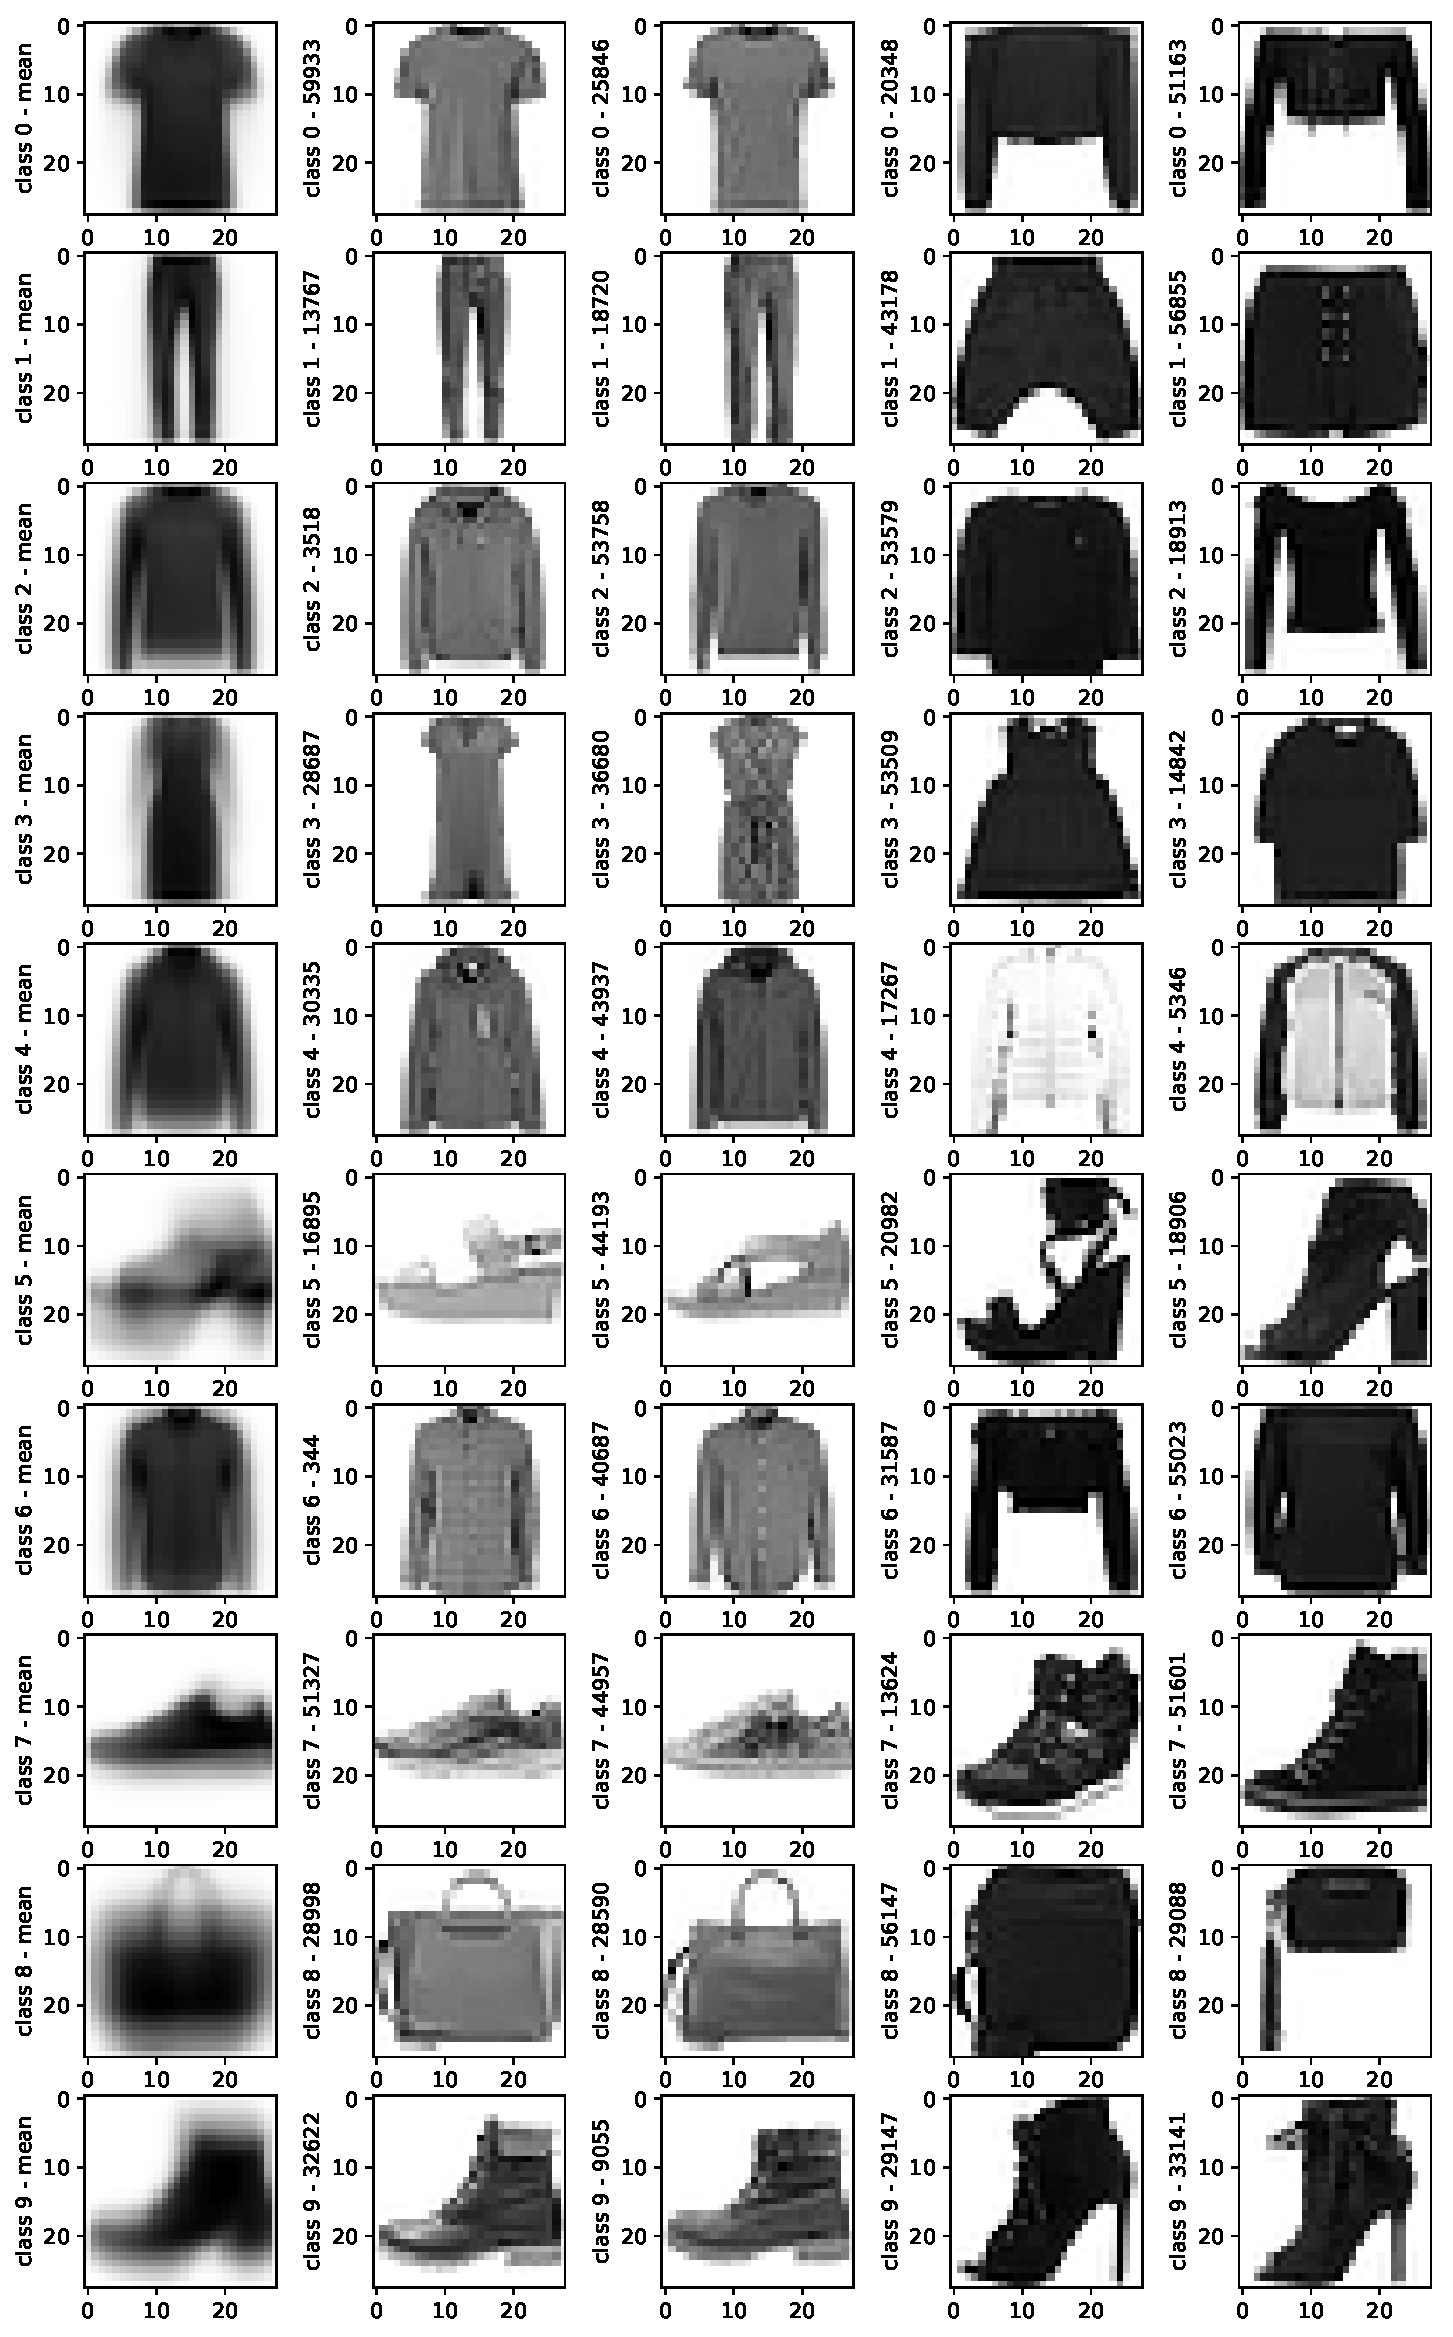
\includegraphics[width=0.6\textwidth]{PCA1.pdf}
    \end{center}
    From the image above, the mean images in each class are blurred and represent main features of objects in each class. We can see that the closest 2 images has similar shape and size to mean image which means majority of samples in this class is similar to them. Mean image and last 2 images have very different shape and size due to different style of design and camera distance. This is why mean image in Class 5 has two different styles mix together and Class 8 has different size bags mix together. Other difference are orientation of objects in images like Class 7 sample 4 and color (darkness and lightness) of objects. It is clear to see 2 images closest to mean image normally has light color while last 2 images normally has dark color except Class 4 last 2 samples.
  \end{answerbox}



   \end{subquestion}

   % 
   % Q1.3
   \begin{subquestion}{(3 points)
       Apply Principal Component Analysis (PCA) to the data of {\tt
         Xtrn\_nm} using
       \href{https://scikit-learn.org/0.19/modules/generated/sklearn.decomposition.PCA.html}{sklearn.decomposition.PCA},
       and report the variances of projected data for the first five principal
       components in a table. 
       Note that you should use {\tt Xtrn\_nm} instead of {\tt Xtrn}.
           } \label{Q1.pca.variance}



    \begin{answerbox}{15em}
      Results are presented in the table below. (variances rounded to 2 decimal places)
      \begin{center}
      \begin{tabular}{|c|c|}
      \hline
      Principle Components & Explained Variance Of Projected Data\\
      \hline
      First & 19.81 \\
      Second & 12.11 \\
      Third & 4.11 \\
      Fourth & 3.38 \\
      Fifth & 2.62 \\
      \hline
      \end{tabular}
      \end{center}
    \end{answerbox}
    


   \end{subquestion}

   %==============================
   % Q1.4
   \begin{subquestion}{(3 points)
       Plot a graph of the cumulative explained variance ratio as a
       function of the number of principal components, $K$, where $1
       \le K \le 784$.
       Discuss the result briefly.
     } \label{Q1.plot.pca.variance}
   

      \begin{answerbox}{30em}
         The image below shows the answer:
         \begin{center}
         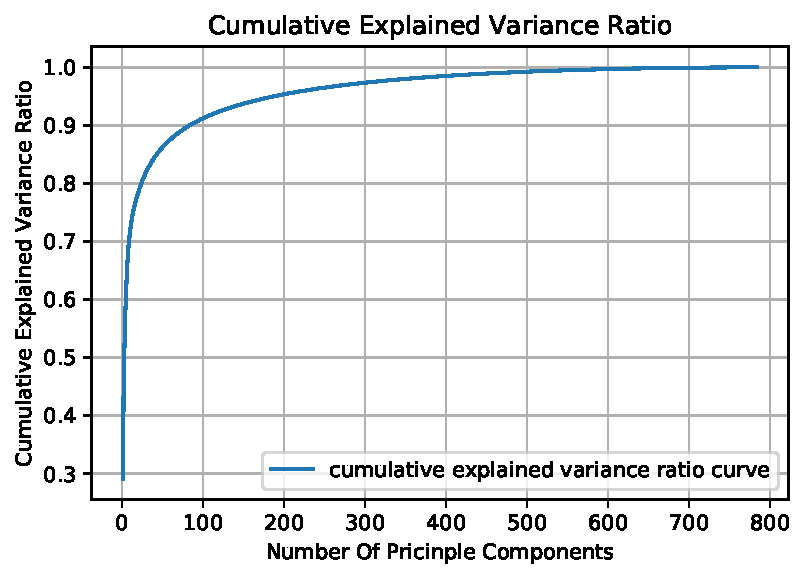
\includegraphics[width=0.6\textwidth]{CEVR.pdf}
         \end{center}
         Cumulative explained variance ratio increases rapidly in the first few of principle components and then increases slowly in the rest of principle components. The ratio increases slower and slower as the number of principle components increase which means principle components become less and less important (component contains less and less variance). The cumulative explained variance ratio over 90\%, 80\% and 70\% are when K=83, 23, 8 respectively. This means that the cumulative sum of variance in the first few principle components has taken up the majority of total variance.
      \end{answerbox}
  


   \end{subquestion}

   %==============================
   % Q1.5
   \begin{subquestion}{(4 points)
      Display the images of the first 10 principal components in
      a 2-by-5 grid, putting the image of 1st principal component on
      the top left corner, followed by the one of 2nd component to the right.
      Discuss your findings briefly.
     } \label{Q1.disp.pca}
   

      \begin{answerbox}{35em}
         The image below shows the answer:
         \begin{center}
         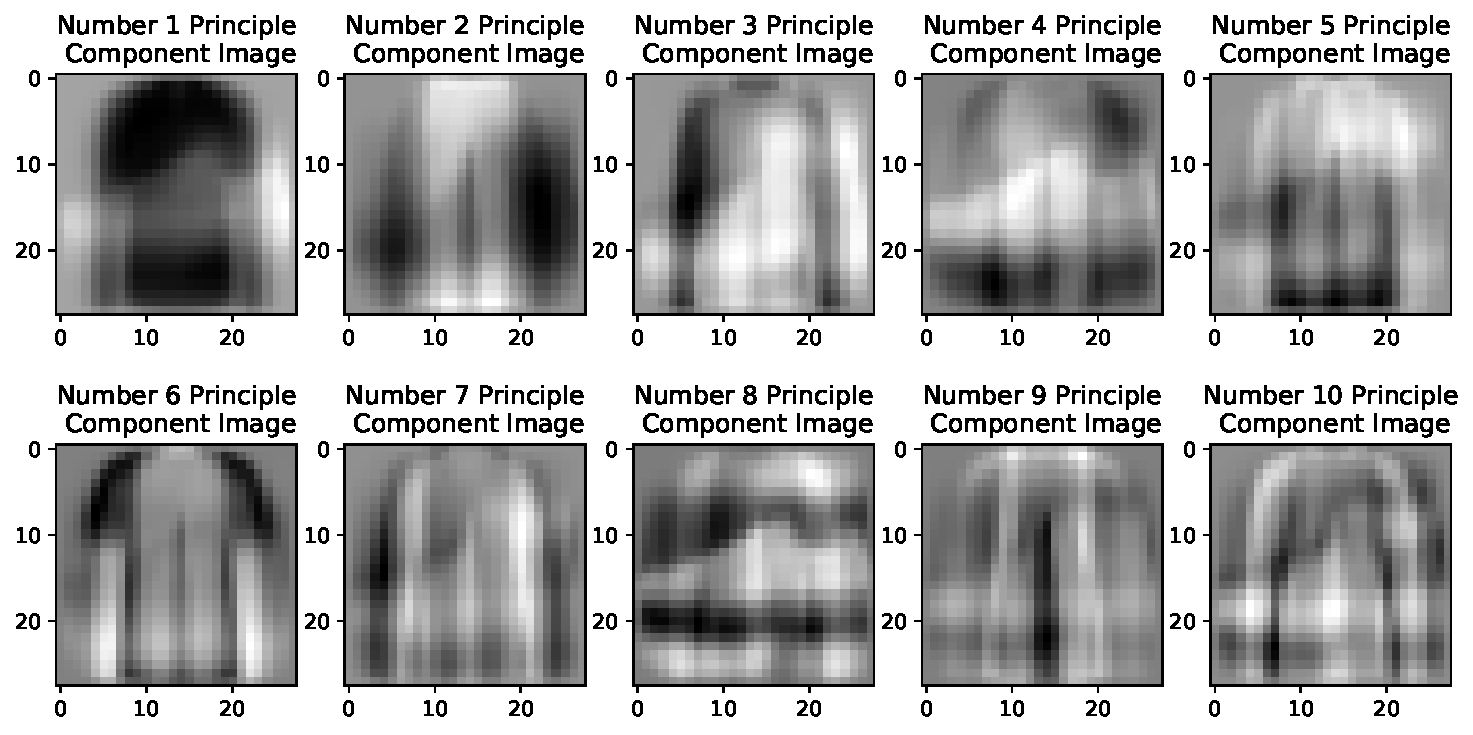
\includegraphics[width=0.8\textwidth]{PCA2.pdf}
         \end{center}
         Each image represents some basis features of different class objects with dark or white color and background always be gray. Each image captures the structure that affects class separability. We can see that the first few principle components mainly distinguish different categories such as shoe, cloth or trousers and features are clear due to large variance on these components. They contain dark or white features that are similar to mean images of some classes. The last few images distinguish details of some classes and becomes blurred due to less variance on these components. White and black area are regions to distinguish something that contributes to a large amount of variance since their value are very positive or very negative which will significantly affect the variance of data which project on eigenimage. And each sample in data set can reform by linear combination of those eigenimages.
      \end{answerbox}
  


   \end{subquestion}

   %==============================
   % Q1.6
   \begin{subquestion}{(5 points)
       Using \texttt{Xtrn\_nm}, 
       for each class and for each number of principal components $K =
       5, 20, 50, 200$, apply dimensionality reduction with PCA to the
       first sample in the class, reconstruct the sample from the
       dimensionality-reduced sample, and 
       report the Root Mean Square Error (RMSE) between the
       original sample in {\tt Xtrn\_nm} and reconstructed one.
     } \label{Q1.6}

     

      \begin{answerbox}{25em}
         Results are presented in the table below. (RMSE rounded to 3 decimal places)
         \begin{center}
         \begin{tabular}{|c|c|c|c|c|}
         \hline
         Class & RMSE(K$=$5) & RMSE(K$=$20) & RMSE(K$=$50) & RMSE(K$=$200)\\
         \hline
         0 & 0.256 & 0.150 & 0.127 & 0.061 \\
         1 & 0.198 & 0.140 & 0.095 & 0.038 \\
         2 & 0.199 & 0.146 & 0.124 & 0.080 \\
         3 & 0.146 & 0.107 & 0.083 & 0.056 \\
         4 & 0.118 & 0.103 & 0.088 & 0.047 \\
         5 & 0.181 & 0.159 & 0.143 & 0.089 \\
         6 & 0.129 & 0.096 & 0.072 & 0.046 \\
         7 & 0.166 & 0.128 & 0.107 & 0.064 \\
         8 & 0.223 & 0.145 & 0.124 & 0.091 \\
         9 & 0.184 & 0.151 & 0.122 & 0.072 \\
         \hline
         \end{tabular}
         \end{center}
    \end{answerbox}
  


   \end{subquestion}
   
   %==============================
   % Q1.7
   \begin{subquestion}{(4 points)
       Display the image for each of the reconstructed samples in
       a 10-by-4 grid, where each row corresponds to a class and
       each row column corresponds to a value of $K=5, \; 20, \; 50, \; 200$.
     } \label{Q1.7}


   

      \begin{answerbox}{52em}
         The image below shows the answer:
         \begin{center}
         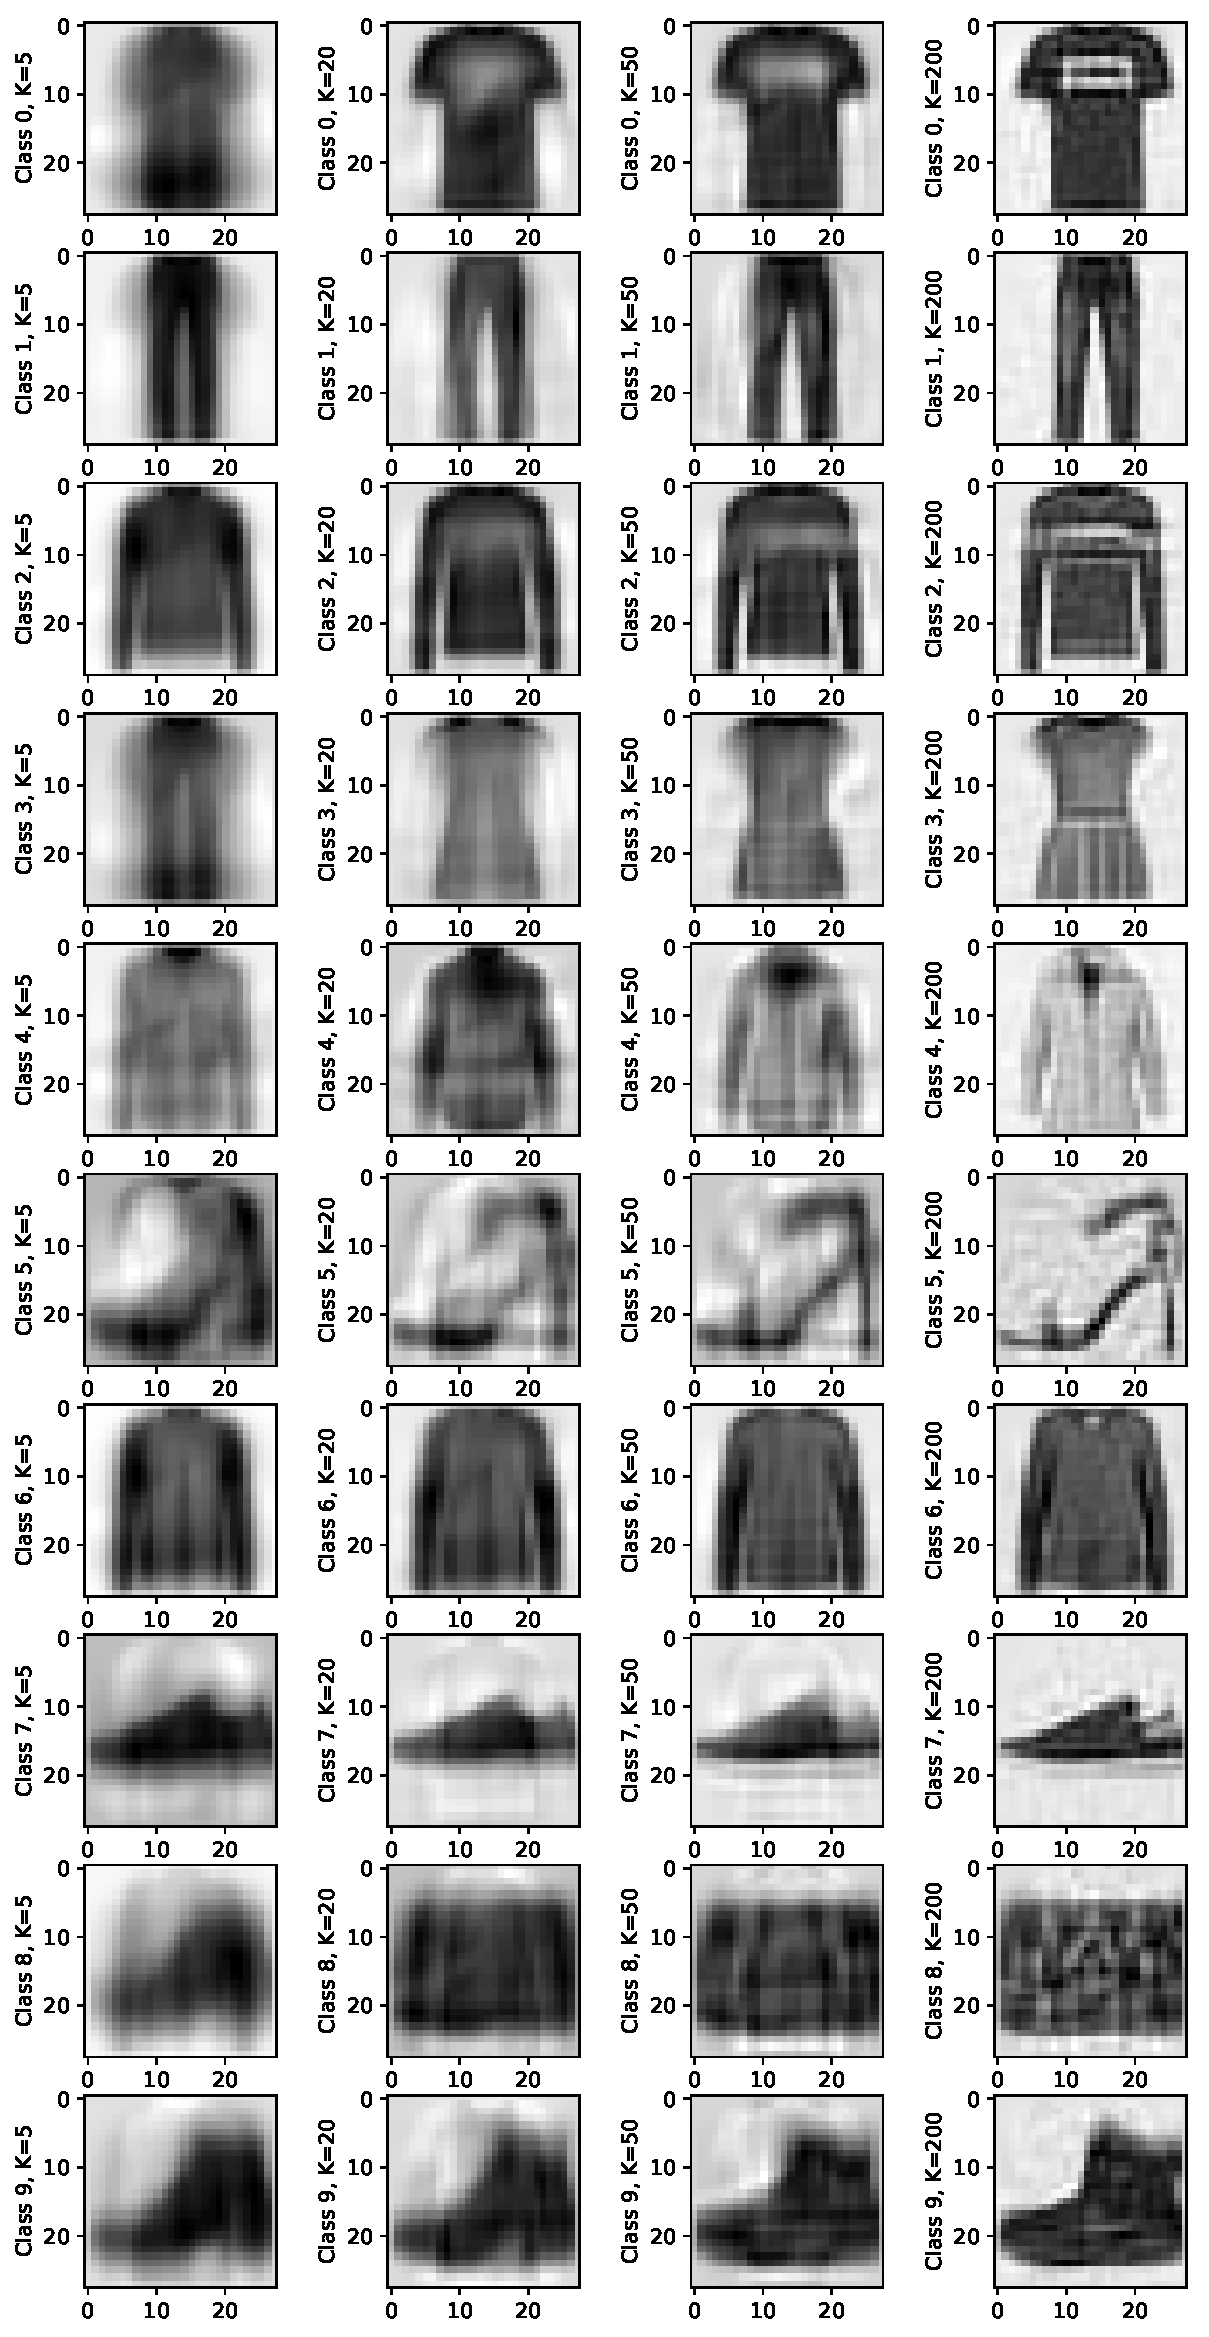
\includegraphics[width=0.5\textwidth]{PCA3.pdf}
         \end{center}
         From image above, images in each class from left to right become more and more clear and we can see more and more details. The image with less number of principle components will be more blurred and easier to be affected by Xmean. We can see some of images in first column has clear Xmean background. They are also similar to mean images which only contains general features. As K becomes larger, more and more specific features appear and image becomes unique rather than only show general features. This is because each image above is made by linear combination of principle components plus a mean vector. The larger the number of principle components to made a image, the more variance will be in the image and image becomes more similar to the original one.
      \end{answerbox}
  


   \end{subquestion}
   %==============================
   %
   %==============================
   % Q1.8
   \begin{subquestion}{(4 points)
       Plot all the training samples (\texttt{Xtrn\_nm}) on the
       two-dimensional PCA plane you obtained in \refQ{Q1.pca.variance}, where each sample is
       represented as a small point with a colour specific to the class of
       the sample.  Use the 'coolwarm' colormap for plotting.
     } \label{Q1.8}


   

      \begin{answerbox}{40em}
         The image below shows the answer:
         \begin{center}
         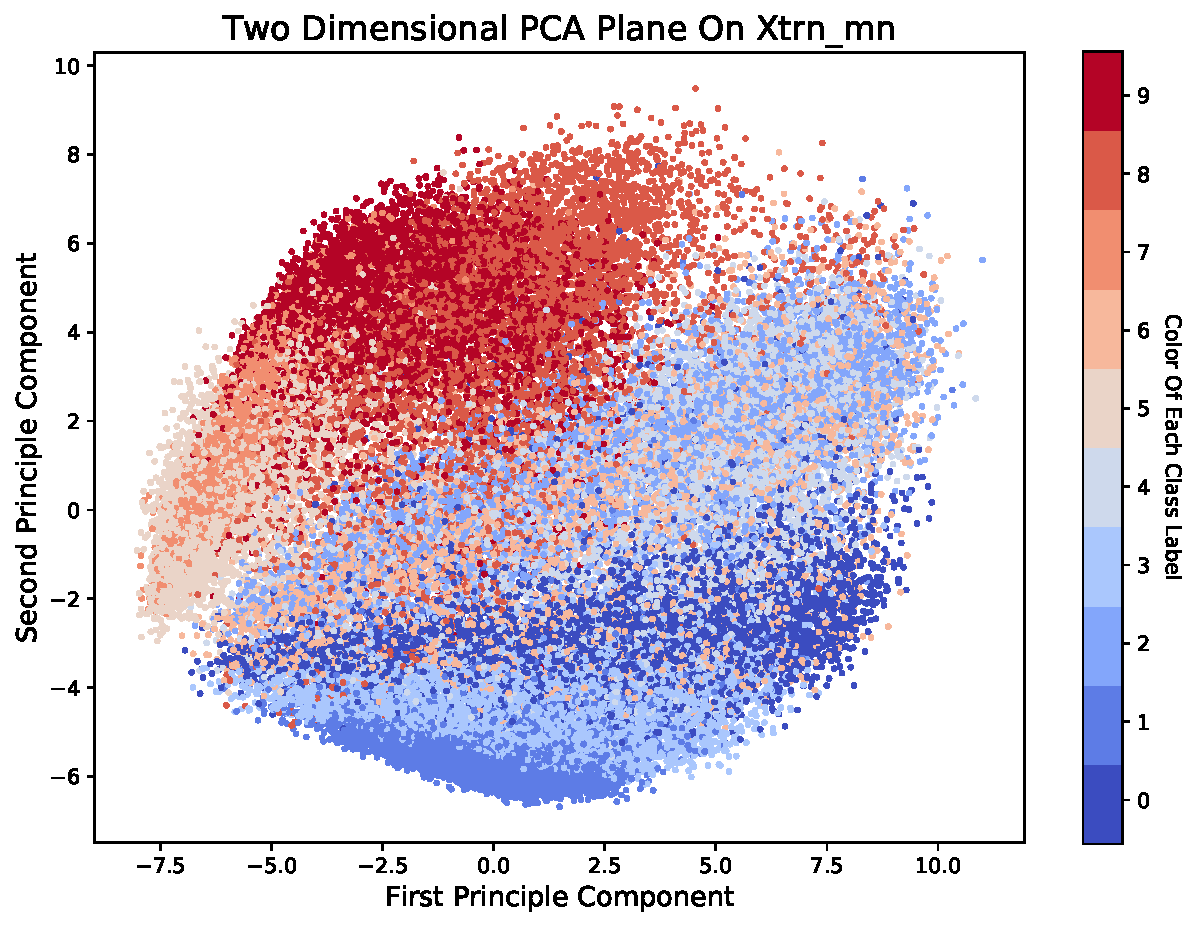
\includegraphics[width=0.7\textwidth]{PCA4.pdf}
         \end{center}
        The points of the same class are grouped together in 2D plane which means general feature in samples of each class are similar to each other. The classes with warm colors and classes with cool colors can be separated by a line from southwest to northeast. We can see that classes with warm colors normally have positive values in second principle component and classes with cool colors normally have negative values in second principle component. This is due to very white trousers and black shoe in eigenimage of second principle component which makes all types of shoes to positive and makes trousers or cloth (cloth is largely overlap with trousers in middle area) to negative. All classes are overlap with each other since 'true dimension' of data are higher than 2 dimensions.
      \end{answerbox}
  


   \end{subquestion}
   %
   %==============================
   

\end{question}
%%%%%%%%%%%%%%%%%%%%%%%%%%%%%%%%%%%%%%%%%%%%%%%%%%%%%%%%%%%%%%%%%%%%%%%%%%%%%%
%============================================================================%
%%%%%%%%%%%%%%%%%%%%%%%%%%%%%%%%%%%%%%%%%%%%%%%%%%%%%%%%%%%%%%%%%%%%%%%%%%%%%%
\clearpage
%
% Question 2
%
\begin{question}{(25 total points) Logistic regression and SVM}

  \questiontext{In this question we will explore 
    classification of image data with logistic regression and support
    vector machines (SVM) and visualisation 
    of decision regions.
  }
  


  \medskip
   %==============================
   % Q2.1
   \begin{subquestion}{(3 points)
       Carry out a classification experiment with
       \href{https://scikit-learn.org/0.19/modules/generated/sklearn.linear\_model.LogisticRegression.html}{multinomial logistic regression},
       and report the classification accuracy and confusion matrix (in
       numbers rather than in graphical representation such as heatmap)
       for the test set.
     } \label{Q2.1}


   

      \begin{answerbox}{30em}
         Classification Accuracy for the test set: 0.840 rounded to 3 decimal places. \\(0.8401 for original output)
         \begin{center}
         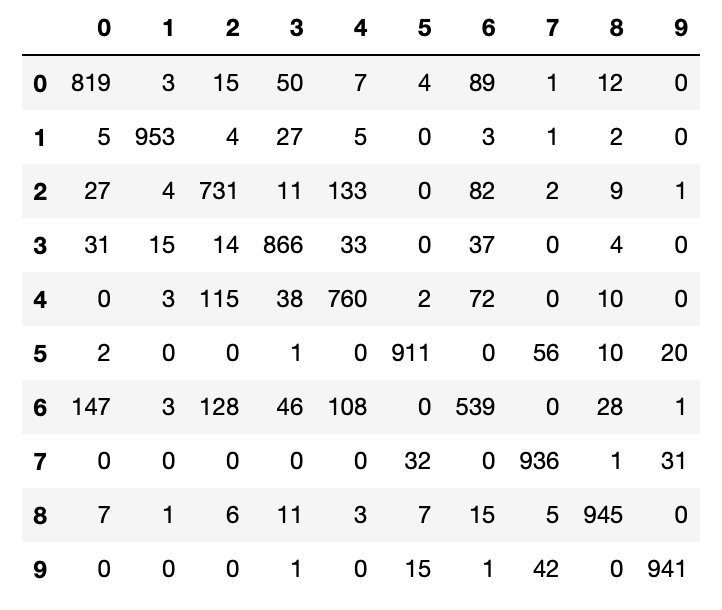
\includegraphics[width=0.6\textwidth]{logistic.png}
         \end{center}
         where left index represents the true labels of each class and upper columns names represent the predicted labels of each class.
      \end{answerbox}
  


   \end{subquestion}
   %
   % ==============================
   %
   %==============================
   % Q2.2
   \begin{subquestion}{(3 points)
       Carry out a classification experiment with
       \href{https://scikit-learn.org/0.19/modules/generated/sklearn.svm.SVC.html}{SVM classifiers}, and report the
       mean accuracy and confusion matrix (in numbers) for the test
       set.
     } \label{Q2.2}


   

      \begin{answerbox}{30em}
         Classification Accuracy for the test set: 0.846 rounded to 3 decimal places.\\(0.8461 for original output)
         \begin{center}
         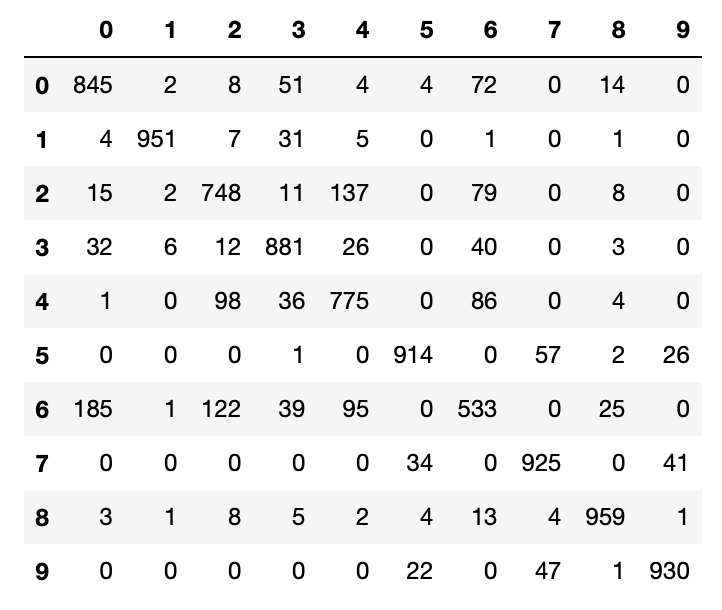
\includegraphics[width=0.6\textwidth]{svm.png}
         \end{center}
         where left index represents the true labels of each class and upper columns names represent the predicted labels of each class.
      \end{answerbox}
  


   \end{subquestion}
   %
   % ==============================
   %
   %==============================
   % Q2.3
   \begin{subquestion}{(6 points)
       We now want to visualise the decision regions for the logistic
       regression classifier we trained in \refQ{Q2.1}.
     } \label{Q2.3}


   

      \begin{answerbox}{35em}
         The image below shows the answer:
         \begin{center}
         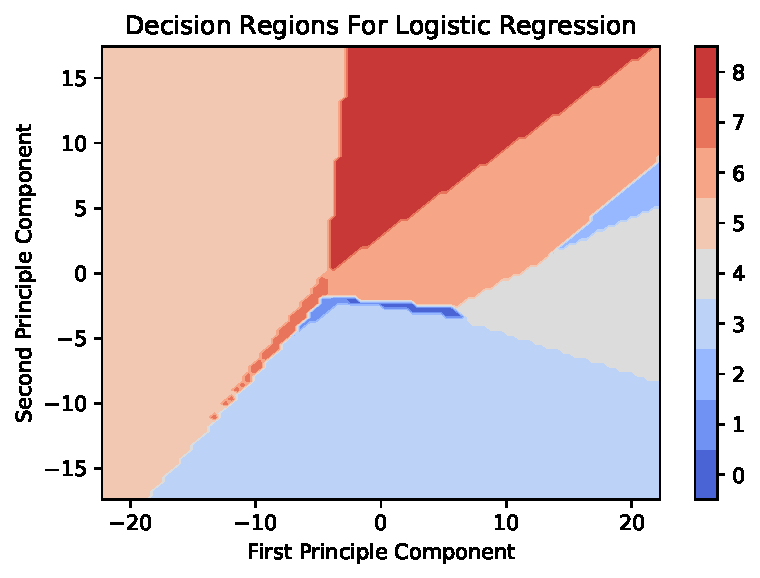
\includegraphics[width=0.6\textwidth]{DR1.pdf}
         \end{center}
         There are just 9 classes occur. The decision regions have straight line decision boundaries since logistic is a linear classifier. Class 1 and 2 and 7 almost disappear and Class 9 is missing since the data in these classes are not linearly separable on original dimensions. From 1.8, we know that those classes in 2D plane overlap with others. Inverse transformation of data that classes are not linear separable in 2D plane to original dimensions still be a 2D plane with non-linear separable data. Therefore, logistic regression which is a linear classifier can not classify these classes well in original dimensions. In general, inverse transformation from 2D data to original dimensions will lost lots of variance (only first two components information remain) so it is difficult for classifier to identify different classes.
      \end{answerbox}
  


   \end{subquestion}
   %
   % ==============================
   %
   %==============================
   % Q2.4
   \begin{subquestion}{(4 points)
       Using the same method as the one above, plot the decision regions for
       the SVM classifier you trained in \refQ{Q2.2}.
       Comparing the result with that you obtained in \refQ{Q2.3}, discuss your
       findings briefly.
     } \label{Q2.4}
   

      \begin{answerbox}{35em}
         The image below shows the answer:
         \begin{center}
         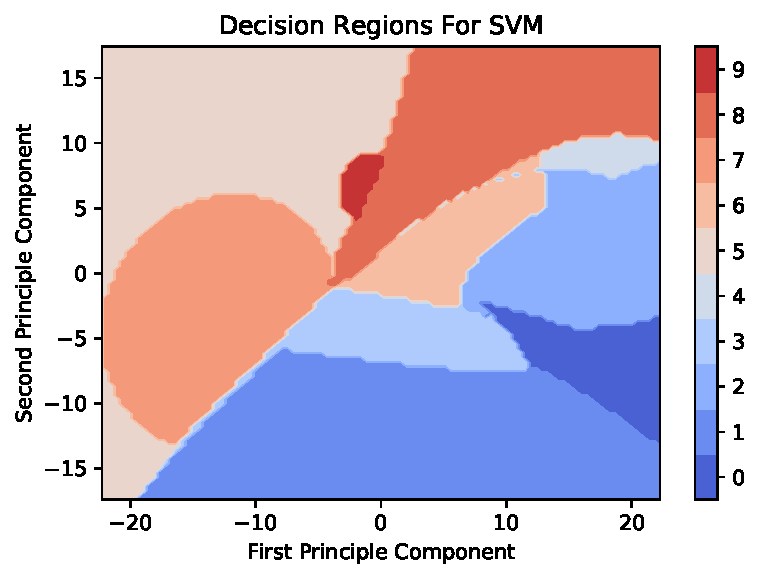
\includegraphics[width=0.6\textwidth]{DR2.pdf}
         \end{center}
         The decision boundaries of SVM classifier are not linear since SVM with Gaussian kernel is non linear classifier. The shape of decision regions in SVM is very different compared to Logistic. Class 9 occur in this region but not occur in Logistic. Class 1,2,7 which almost disappear in Logistic have become larger. This is because data is not linear separable on original dimensions (inverse transformation of non linearly separable data in 2D plane to original dimensions are still be non linearly separable 2D plane in high dimensions) and SVM classify data by using Gaussian kernel to find a hyperplane in another vector space to make non linearly separable data separable. That is why SVM has better decision regions than Logistic Regression.
      \end{answerbox}
  


   \end{subquestion}
   %
   % ==============================
   %

   %==============================
   % Q2.5
   \begin{subquestion}{(6 points)
       We used default parameters for the SVM in \refQ{Q2.2}.
       We now want to tune the parameters by using cross-validation.
       To reduce the time for experiments, you pick up the first 1000
       training samples from each class to create \texttt{Xsmall}, so that \texttt{Xsmall}
       contains 10,000 samples in total. Accordingly, you create
       labels, \texttt{Ysmall}.
     } \label{Q2.5}


   

      \begin{answerbox}{30em}
         The image below shows the answer:
         \begin{center}
         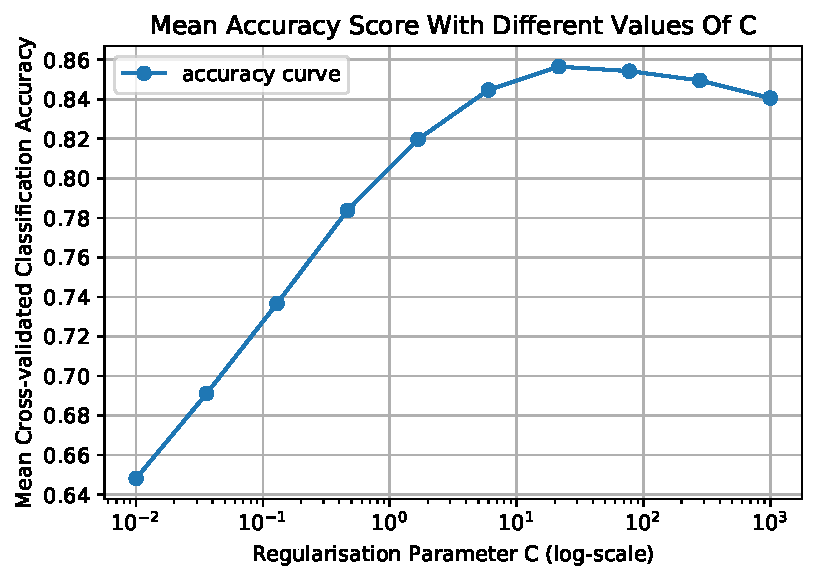
\includegraphics[width=0.6\textwidth]{MASC.pdf}
         \end{center}
         The highest obtained mean accuracy score is 0.857 rounded to 3 decimal places.\\
         The value of C corresponds to this accuracy is 21.54 rounded to 2 decimal places.
      \end{answerbox}
  


   \end{subquestion}
   %
   % ==============================
   %
   %==============================
   % Q2.6
   \begin{subquestion}{(3 points)
       Train the SVM classifier on the whole training set by using the
       optimal value of $C$ you found in \refQ{Q2.5}. 
     } \label{Q2.6}


       

      \begin{answerbox}{10em}
      Results are presented in the table below. (rounded to 3 decimal places)
         \begin{center}
         \begin{tabular}{|c|c|c|}
         \hline
         Training Accuracy & Test Accuracy \\
         \hline
         0.908 & 0.877 \\
         \hline
         \end{tabular}
         \end{center}
      Original result on training set by using optimal value of C is 0.9084.\\
      Original result on test set by using optimal value of C is 0.8765.
      \end{answerbox}
  


   \end{subquestion}
   %
   % ==============================
   %
%
%

\end{question}
%%%%%%%%%%%%%%%%%%%%%%%%%%%%%%%%%%%%%%%%%%%%%%%%%%%%%%%%%%%%%%%%%%%%%%%%%%%%%%
%============================================================================%
%%%%%%%%%%%%%%%%%%%%%%%%%%%%%%%%%%%%%%%%%%%%%%%%%%%%%%%%%%%%%%%%%%%%%%%%%%%%%%
\clearpage
%
% Question 3
%

\begin{question}{(20 total points) Clustering and Gaussian Mixture Models}  


  \questiontext{In this question we will explore K-means clustering,
    hierarchical clustering, and GMMs.
  }
  


  \medskip
   %==============================
   % Q3.1
   \begin{subquestion}{(3 points)
       Apply k-means clustering on {\tt Xtrn} for $k = 22$, where we use
       \href{https://scikit-learn.org/0.19/modules/generated/sklearn.cluster.KMeans.html}{sklearn.cluster.KMeans}
       with the parameters {\tt n\_clusters=22} and {\tt random\_state=1}.
       Report the sum of squared distances of samples to their closest
       cluster centre, and the number of samples for each cluster.
     } \label{Q3.1}
   

      \begin{answerbox}{35em}
         Results are presented in the table below.
         \begin{center}
         \begin{tabular}{|c|c|c|}
         \hline
         Cluster Number & Number Of Samples \\
         \hline
         0 & 1018 \\
         1 & 1125 \\
         2 & 1191 \\
         3 & 890 \\
         4 & 1162 \\
         5 & 1332 \\
         6 & 839 \\
         7 & 623 \\
         8 & 1400 \\
         9 & 838 \\
         10 & 659 \\
         11 & 1276 \\
         12 & 121 \\
         13 & 152 \\
         14 & 950 \\
         15 & 1971 \\
         16 & 1251 \\
         17 & 845 \\
         18 & 896 \\
         19 & 930 \\
         20 & 1065 \\
         21 & 1466 \\
         \hline
         \end{tabular}
         \end{center}
         Sum of squared distances of samples to their closest cluster centre is 38185.82 rounded to 2 decimal places.
      \end{answerbox}
  


   \end{subquestion}
   %
   % ==============================
   %
   %==============================
   % Q3.2
   \begin{subquestion}{(3 points)
       Using the training set only,
       calculate the mean vector for each language, and plot the mean
       vectors of all the 22 languages on a 2D-PCA plane, where you
       apply PCA on the set of 22 mean vectors without applying
       standardisation.  
       On the same figure, plot the cluster centres obtained in \refQ{Q3.1}.
     } \label{Q3.2}

   

      \begin{answerbox}{35em}
         The image below shows the answer:
         \begin{center}
         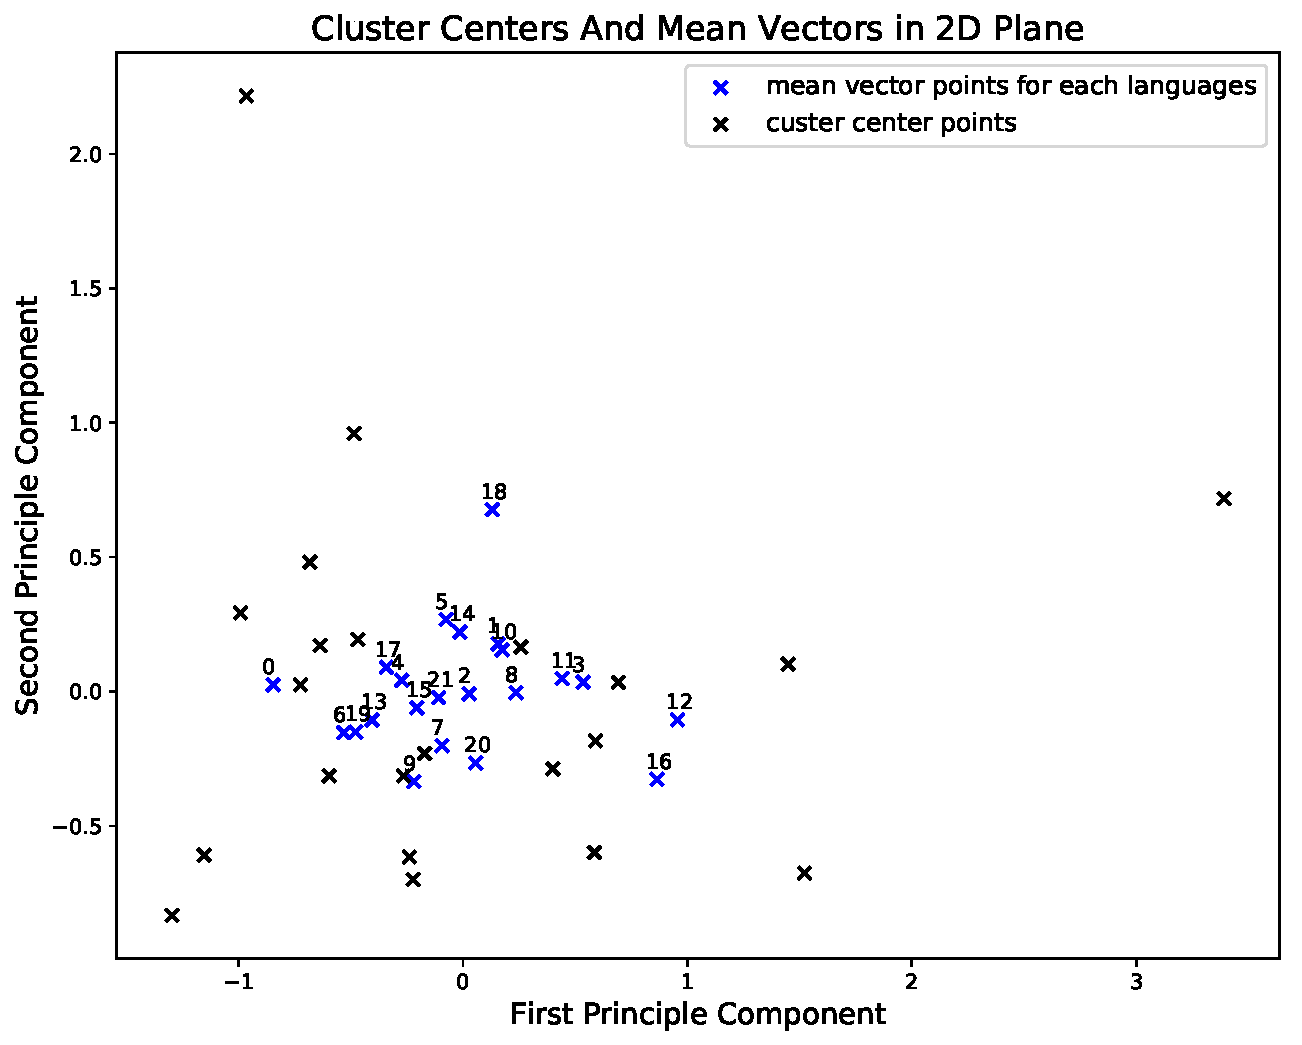
\includegraphics[width=0.6\textwidth]{Cluster1.pdf}
         \end{center}
         From image above, we can see that mean vector of each language projected into 2D plane close to each other. This means that the general feature of speech information in different languages are similar. But mean vectors and cluster centers are not similar. Cluster centers widely spread while mean vectors group into a small region. Some cluster centers are far away from other points. This is because some clusters has been dragged by outliers. Different initial position of centers will results in different position of cluster centers because Kmeans is sensitive to outliers. So it cannot guarantee the positions of 22 clusters will get best match with 22 languages. Kmeans is unsupervised learning so we cannot ensure which cluster belongs to which language.
      \end{answerbox}
  


   \end{subquestion}
   %
   % ==============================
   %
   %==============================
   % Q3.3
   \begin{subquestion}{(3 points)
       We now apply hierarchical clustering on the training data set
       to see if there are any structures in the spoken languages.
     } \label{Q3.3}


     

      \begin{answerbox}{35em}
         The image below shows the answer:
         \begin{center}
         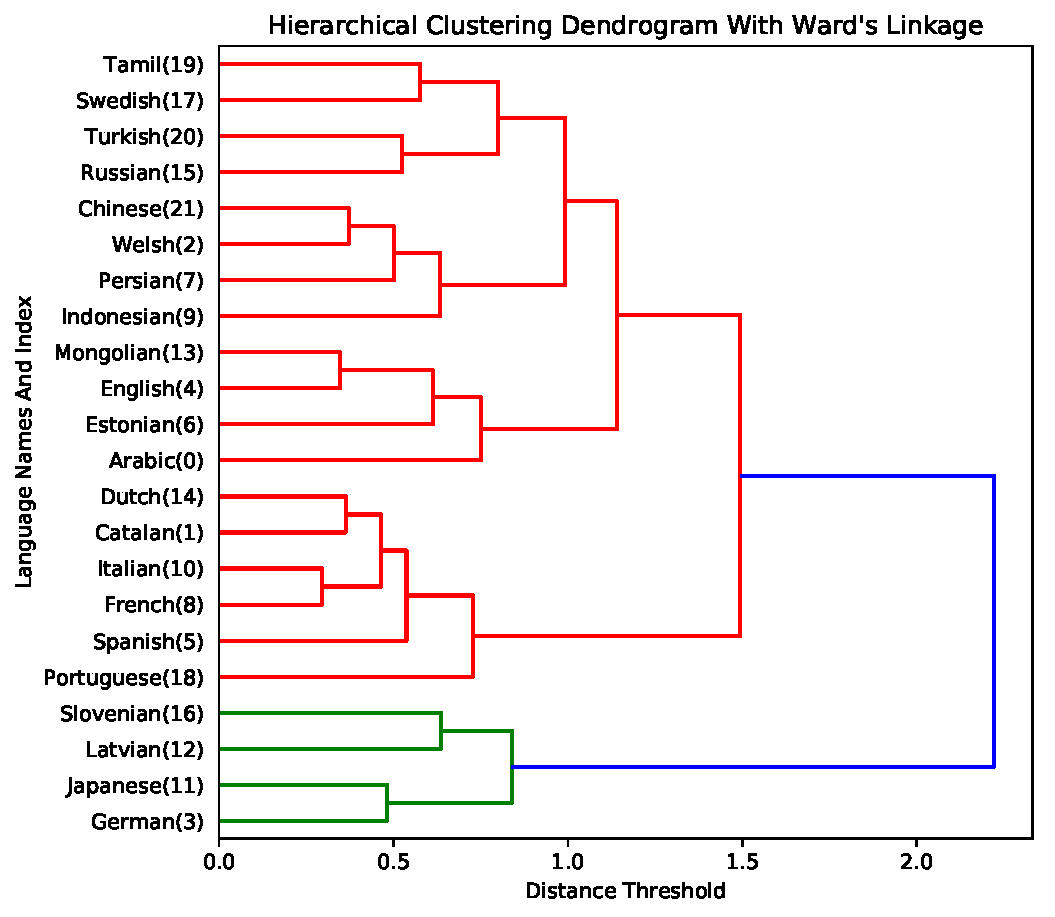
\includegraphics[width=0.6\textwidth]{Cluster2.pdf}
         \end{center}
         Ward Linkage measures distance of clusters by minimizing the change of within-cluster variances before and after merge. So it forms small groups first and combines them later. Ward can group the languages in the same geographical region into the same cluster such as European language cluster between Dutch and Portuguese. Those languages may have the same ancestor language, so they have similar speech information. Some of languages are in different regions but cluster together such as Chinese and Welsh, Japanese and German. This may because they have similar tone of voice.
      \end{answerbox}
  


   \end{subquestion}
   %
   % ==============================
   %
   %==============================
   % Q3.4
   \begin{subquestion}{(5 points)
       We here extend the hierarchical clustering done in \refQ{Q3.3} by
       using multiple samples from each language.
     } \label{Q3.4}


   

      \begin{answerbox}{50em}
      The images below show the answer:\\
      
         \begin{tabular}{ ll }
         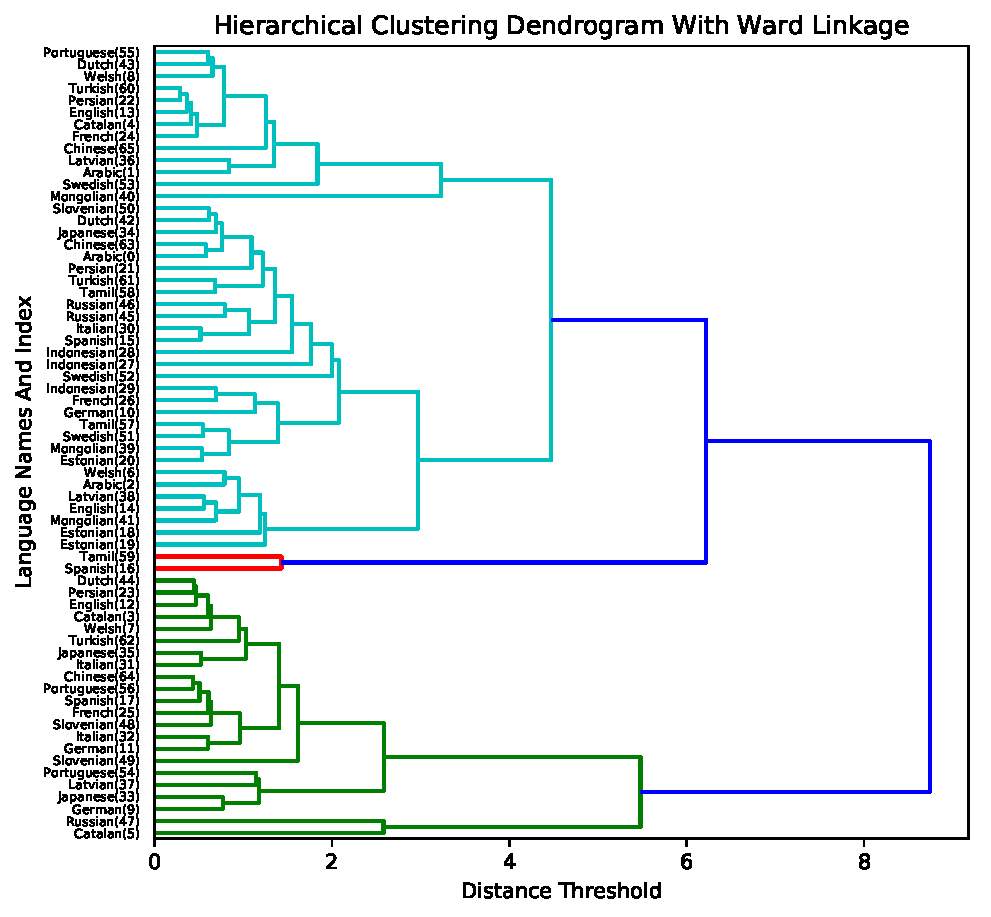
\includegraphics [width=0.48\textwidth]{Cluster-ward.pdf}
         &
         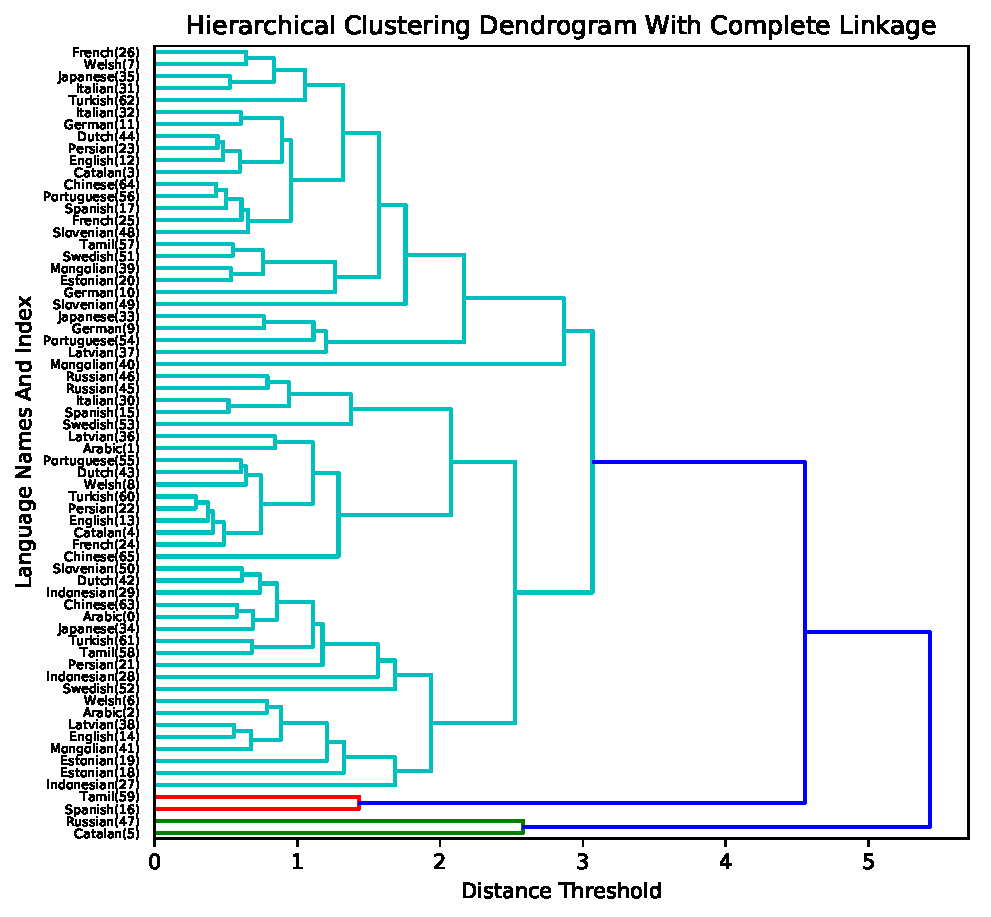
\includegraphics [width=0.48\textwidth]{Cluster-complete.pdf} \end{tabular}
         \begin{center}
         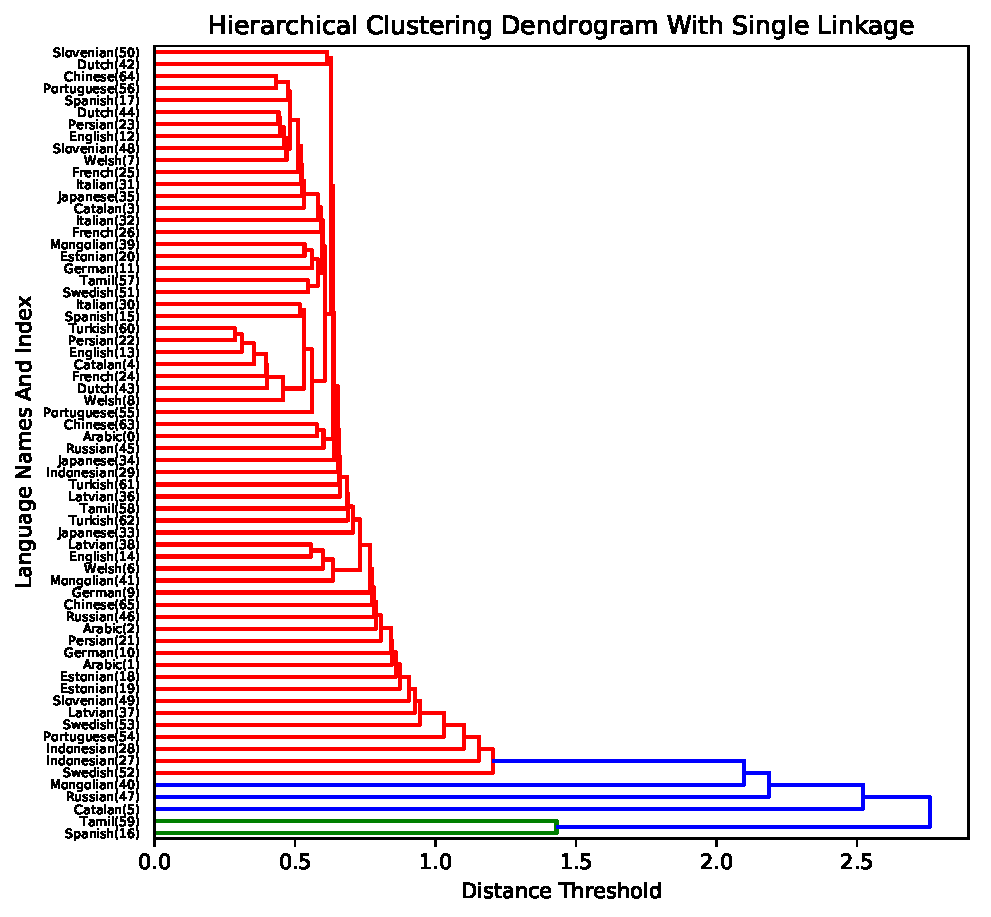
\includegraphics[width=0.48\textwidth]{Cluster-single.pdf}
         \end{center}
      Ward and Complete has similar cluster pattern that forces spherical clusters but Single forces a long chains. This difference is caused by different similarity measure between clusters. Ward Linkage measures similarity by within-cluster variance change before and after merge. Complete Linkage measures similarity by distance between furthest elements in clusters. Single Linkage measures similarity by distance between closest elements in clusters. We can see that there are two outlier clusters (47,5 and 59,16). This is caused by outliers in their language samples drag the centers in KMeans. The threshold distance are different. maximum distance in Single is the smallest, in Ward is the largest and in Complete is middle. 
      \end{answerbox}
  


   \end{subquestion}
   %
   % ==============================
   %
   %==============================
   % Q3.5
   \begin{subquestion}{(6 points)
       We now consider Gaussian mixture model (GMM), whose
       probability distribution function (pdf) is given as
       a linear combination of Gaussian or normal distributions, i.e.,
     } \label{Q3.5}




      \begin{answerbox}{30em}
         The images below show the answer:
         \begin{center}
         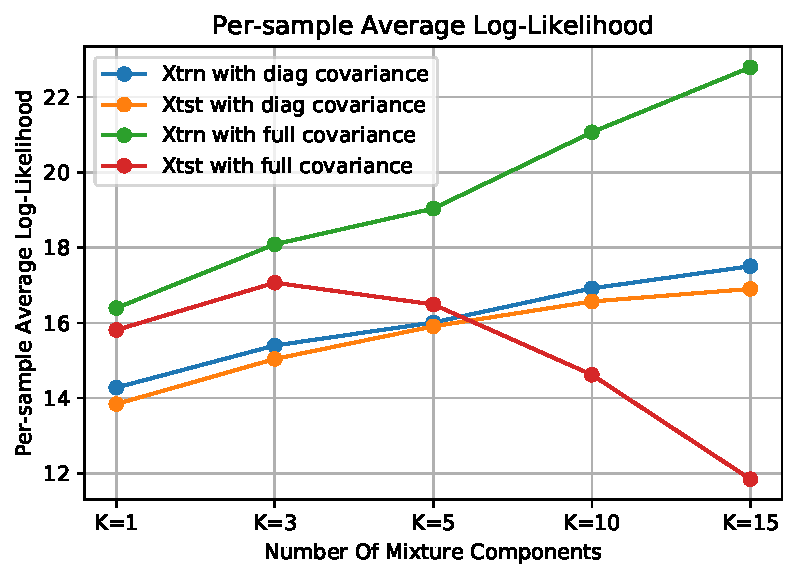
\includegraphics [width=0.43\textwidth]{Mixture.pdf} \end{center}
         \resizebox{\textwidth}{10mm}{
         \begin{tabular}{|c|c|c|c|c|c|c|c|c|c|c|c|}
         \hline
         & K=1 & K=1 & K=3 & K=3 & K=5 & K=5 & K=10 & K=10 & K=15 & K=15\\ 
         \hline
         & full & diag & full & diag & full & diag & full & diag & full & diag \\
         Xtrn & 16.39 & 14.28 & 18.09 &15.40& 19.04&16.01&21.06&16.92&22.79&17.50\\
         Xtst & 15.81 & 13.84 & 17.07 & 15.04&16.49&15.91&14.62&16.57&11.85&16.90\\
         \hline
         \end{tabular}}\\
         \newline
         For GMM with full covariance matrix, the likelihood of training data increases when K increases but the likelihood of testing data decreases after K=3 because more components added shrink size of Gaussians so the model will be more likely to be overfitting. Both likelihood of training and testing data in GMM with diagonal covariance matrix increase when K increases and likelihood values are similar. This is because diagonal will lose information provided by correlation of dimensions of data and make dimensions of data indepedent to each other. Therefore the results will be less affected by increase in components.
      \end{answerbox}
  


   \end{subquestion}
   %
   %==============================

   % ==============================
   
\end{question}
\end{document}
